\documentclass[12pt,aspectratio=169,envcountset]{beamer}
\usepackage{
  amsfonts,amsmath,amssymb,
  derivative,
  epigraph,
  geometry,
  isomath,
  listings,
  mathtools,
  parskip,
  tikz
}
\usepackage[framed,numbered]{matlab-prettifier}
\usepackage{algorithmic,algorithm}
\usepackage[backend=bibtex,style=authoryear]{biblatex}
\addbibresource{../na_refs.bib}
\usepackage{hyperref}
\usetikzlibrary{arrows.meta,calc,shapes.geometric,positioning}
\tikzset {
  >=Stealth,
  every node/.style={font=\small},
}

\hypersetup{
  colorlinks=true,
  allcolors=ujorange
}

\usetheme{Hoepoe}
\usefonttheme[onlymath]{serif}
\beamertemplatenavigationsymbolsempty
\setbeamertemplate{footline}[frame number]
%\setbeamertemplate{footline}[page number]
\setbeamertemplate{theorems}[numbered]
\setbeamertemplate{definitions}[numbered]
\setbeamertemplate{examples}[numbered]
\AtBeginSection[]{
  \begin{frame}
  \vfill
  \centering
  \begin{beamercolorbox}[sep=8pt,center,shadow=true,rounded=true]{title}
    \usebeamerfont{title}\insertsectionhead\par%
  \end{beamercolorbox}
  \vfill
  \end{frame}
}

\def\modulecode{APM02B2}
\def\modulename{Introduction to Numerical Analysis}
%\def\topicno{00}
\def\topicname{Bisection Method}
\title{\modulecode\ \modulename}
\subtitle{\topicname}
\title[\modulecode]{\modulecode\ \modulename}
\author[Dr Anderson]{Dr K. D. Anderson}
\institute[UJ]{University of Johannesburg}
\def\logo{\includegraphics[width=100px]{../../img/UJ_logo.png}}
\titlegraphic{\logo}
\date{}

\renewcommand{\vec}{\vectorsym}
\providecommand{\mat}{\matrixsym}
\DeclarePairedDelimiter{\abs}{\lvert}{\rvert}
\DeclarePairedDelimiter{\norm}{\lVert}{\rVert}
\providecommand{\defeq}{\coloneqq}

\begin{document}
\frame{\maketitle}
\frame{%
  \tableofcontents 
  \epigraph{
    The purpose of computing is insight, not numbers.
  }{\textit{Richard W. Hamming}}
}
%\frame{%
%  \tableofcontents
%  \epigraph{
%    Numerical analysis is the study of algorithms for solving problems of
%    continuous mathematics, by which we mean problems involving real or complex
%    variables.
%  }{\textit{Lloyd N. Trefethen}}
%}

%\section{Introduction}
%\begin{frame}{Introduction}
%  Equations of various kinds arise in a range of applications.
%
%  Some equations are simple and easy to solve.
%
%  Consider, for example, the \emph{linear equation}
%  \begin{equation} \label{eq:linear-eq}
%    ax + b = 0,
%  \end{equation}
%  which has the solution
%  \begin{equation} \label{eq:linear-eq-soln}
%    x^* = -\frac{b}{a}, \quad
%    a \neq 0.
%  \end{equation}
%\end{frame}
%
%\begin{frame}{Introduction}
%  Some equations are \emph{nonlinear}.
%
%  The simplest example of a nonlinear equation is the \emph{quadratic equation}
%  \begin{equation} \label{eq:quadratic-eq}
%    ax^2 + bx + c = 0,
%  \end{equation}
%  which has the solution
%  \begin{equation} \label{eq:quadratic-eq-soln}
%    x^*_1 = \frac{-b + \sqrt{b^2 - 4ac}}{2a}, \quad
%    x^*_2 = \frac{-b - \sqrt{b^2 - 4ac}}{2a}, \quad
%    a \neq 0.
%  \end{equation}
%\end{frame}

\section{Root-finding Methods}
\begin{frame}{Problem Statement}
  Let $I \subset \mathbb{R}$ be an interval of the real numbers and $f : I \to
  \mathbb{R}$ be continuous on $I$.

  Generally, we assume that $I$ is a bounded and closed interval.
  That is,
  \[
    I = [a, b],
  \] 
  where $a, b \in \mathbb{R}$ such that $a < b$ (this
  guarantees that $I$ is not empty).

  \begin{block}{Problem}
  Consider the general equation
  \begin{equation} \label{eq:root-eq}
    f(x) = 0.
  \end{equation}
  We wish to find all $x^* \in I$ that satisfy equation \eqref{eq:root-eq}.
  These $x^*$ are called the \emph{roots of the function $f$}.
  \end{block}
\end{frame}

\begin{frame}{Root-finding Methods}
  \emph{Root-finding methods} are \emph{iterative methods} to approximate the
  roots of $f$, that is, they are methods to approximate the solutions to
  equation \eqref{eq:root-eq}.

  An \emph{iterative method} is a mathematical procedure that uses an
  \emph{initial value} $x_0$ to generate a sequence   
  \[
    (x_k)_{k=0}^\infty = (x_0, x_1, x_2, \dotsc)
  \]
  of improving approximate solutions to a problem.

  If $x^*$ is a root of $f$, then ideally we want
  \[
    \lim_{k\to\infty} x_k = x^*.
  \]
  However, in practice, we shall not let $k \to \infty$ and only consider a
  finite number of elements of the sequence.
\end{frame}

\begin{frame}{Iterative Method}
  Iterative methods are usually defined by a \emph{recurrence relation}
  \begin{equation} \label{eq:recurrence-relation-1st-order}
    x_k = \psi(x_{k-1})
  \end{equation}
  or
  \begin{equation} \label{eq:recurrence-relation-k-order}
    x_k = \Psi(x_0, x_1, x_2, \dotsc, x_{k-1}),
  \end{equation}
  where $\psi$ is some function describing the functional relationship
  between $x_k$ and other values in the recurrence and is established by the
  particular iterative method.

  For the recurrence relation \eqref{eq:recurrence-relation-1st-order} we
  need to specify a single initial condition $x_0$, also called the
  \emph{initial value}.

  For the recurrence relation \eqref{eq:recurrence-relation-k-order} we would
  need to specify $k - 1$ initial values.

  Most methods in numerical analysis are of the form
  \eqref{eq:recurrence-relation-1st-order}.
\end{frame}

\section{Bisection Method}
\begin{frame}{Bisection Method}
  The \emph{bisection method}'s name derives from what it does:
  ``\href{https://dictionary.cambridge.org/dictionary/english/bisect}{bisect}''
  means ``to divide something in two, usually equal, parts''.

  It is an iterative method for approximating the roots of a general functional
  equation \eqref{eq:root-eq}.
  It is a robust method but converges slowly.

  It is also known by the following names: interval halving method, binary
  search method\footnote{Not to be confused with binary search from Computer
  Science.}, and dichotomy method.

  Out of all the root-finding methods we are going to study, it requires the
  least information about $f$---it only requires that 
  \begin{itemize}
    \item $f$ be continuous on an interval which contains the root, and
    \item the sign of $f$ at two points on this interval.
  \end{itemize}
\end{frame}

\begin{frame}{Bisection Method}{Insight}
  \begin{columns}[onlytextwidth]
    \begin{column}{.4\textwidth}
      \begin{center}
        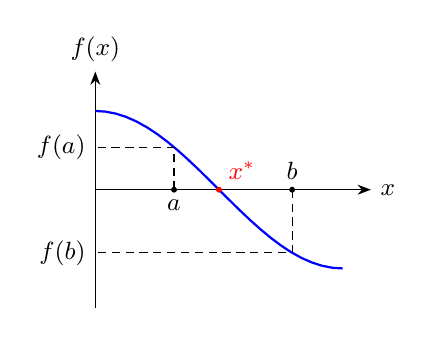
\begin{tikzpicture}
          \coordinate (f1) at (1,{cos(1 r)});
          \coordinate (f1x) at (1,0);
          \coordinate (f1y) at (0,{cos(1 r)});
          \coordinate (f2) at (2.5,{cos(2.5 r)});
          \coordinate (f2x) at (2.5,0);
          \coordinate (f2y) at (0,{cos(2.5 r)});
          \draw[->] (0,0) -- (7/2,0) node[right]{$x$};
          \draw[->] (0,-3/2) -- (0,3/2) node[above]{$f(x)$};
          \draw[blue,thick,domain=0:pi] plot(\x, {cos(\x r)});
          \node at (pi/2,0)[above right,red]{$x^*$};
          \draw[densely dashed] (f1x) -- (f1) -- (f1y);
          \draw[densely dashed] (f2x) -- (f2) -- (f2y);
          \node at (f1x)[below]{$a$};
          \node at (f2x)[above]{$b$};
          \node at (f1y)[left]{$f(a)$};
          \node at (f2y)[left]{$f(b)$};
          \filldraw[red] (pi/2,0) circle[radius=.3mm];
          \filldraw (1,0) circle[radius=.3mm];
          \filldraw (2.5,0) circle[radius=.3mm];
        \end{tikzpicture}
      \end{center}
    \end{column}
    \begin{column}{.5\textwidth}
      The bisection method relies on a simple insight: if an interval $I =
      [a,b]$ can be found such that
      \[
        f(a)f(b) < 0,
      \]
      and $f$ is continuous on this interval, then $f$ has \emph{at least one
      real root $x^*$} on the interval.
      \vskip\baselineskip
      This follows from the intermediate value theorem.
    \end{column}
  \end{columns}
\end{frame}

\begin{frame}{Bisection Method}{Methodology}
  \begin{columns}[onlytextwidth]
    \begin{column}{.4\textwidth}
      \begin{center}
        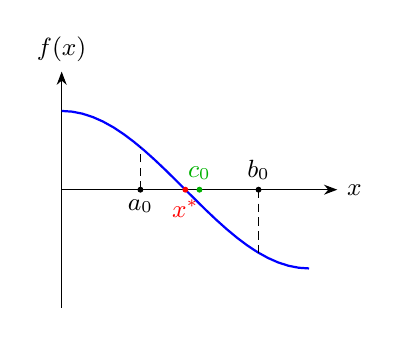
\begin{tikzpicture}
          \coordinate (f1) at (1,{cos(1 r)});
          \coordinate (f1x) at (1,0);
          \coordinate (f1y) at (0,{cos(1 r)});
          \coordinate (f2) at (5/2,{cos(5/2 r)});
          \coordinate (f2x) at (5/2,0);
          \coordinate (f2y) at (0,{cos(5/2 r)});
          \draw[->] (0,0) -- (7/2,0) node[right]{$x$};
          \draw[->] (0,-3/2) -- (0,3/2) node[above]{$f(x)$};
          \draw[blue,thick,domain=0:pi] plot(\x, {cos(\x r)});
          \draw[densely dashed] (f1x) -- (f1);
          \draw[densely dashed] (f2x) -- (f2);
          \node at (f1x)[below]{$a_0$};
          \node at (f2x)[above]{$b_0$};
          %\node at (f1y)[left]{$f(a)$};
          %\node at (f2y)[left]{$f(b)$};
          \node at (pi/2,0)[below,red]{$x^*$};
          \node at (7/4,0)[above,green!70!black]{$c_0$};
          \filldraw[red] (pi/2,0) circle[radius=.3mm];
          \filldraw (1,0) circle[radius=.3mm];
          \filldraw (5/2,0) circle[radius=.3mm];
          \filldraw[green!70!black] (7/4,0) circle[radius=.3mm];
        \end{tikzpicture}
      \end{center}
    \end{column}
    \begin{column}{.5\textwidth}
      Let $I = [a,b] = [a_0, b_0] = I_0$.
      \vskip\baselineskip
      Calculate the midpoint of $I_0$:
      \[
        {\color{green!70!black} c_0} = \frac{a_0 + b_0}{2}.
      \]
      This value $c_0$ is considered the initial approximation to the root $x^*$.
    \end{column}
  \end{columns}
\end{frame}

\begin{frame}{Bisection Method}{Methodology}
  Next, we compare $f(a)f(c_0)$ and $f(c_0)f(b)$:
    
  \begin{itemize}
    \item If $f(a)f(c_0) < 0$, then $x^* \in [a_0,c_0]$ and we set $I_1 =
      [a_1,b_1] = [a_0,c_0]$.  
    \item If $f(c_0)f(b) < 0$, then $x^* \in [c_0,b_0]$ and we set $I_1 =
      [a_1,b_1] = [c_0,b_0]$.
  \end{itemize}
  Then we calculate $c_1 = \frac{1}{2}(a_1 + b_1)$. 
  \begin{center}
    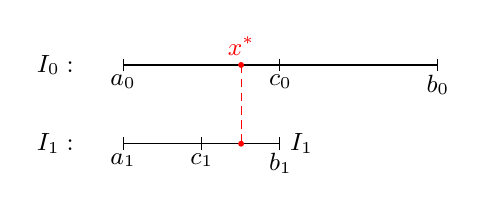
\begin{tikzpicture}
      \draw[|-|] (0,0) -- (2,0) node[below]{$c_0$};
      \draw[-|] (2,0) -- (4,0);
      \node at (0,0)[below]{$a_0$};
      \node at (4,0)[below]{$b_0$};

      \draw[|-|] (0,-1) node[below]{$a_1$} -- (1,-1) node[below]{$c_1$};
      \draw[-|] (1,-1) -- (2,-1) node[below]{$b_1$}
      node[right]{$I_1$};

      \node at(3/2,0)[above,red]{$x^*$};
      \filldraw[red] (3/2,0) circle[radius=.3mm];
      \filldraw[red] (3/2,-1) circle[radius=.3mm];
      \draw[densely dashed,red] (3/2,0) -- (3/2,-1);

      \node at(0,0)[left=5mm]{$I_0:$};
      \node at(0,-1)[left=5mm]{$I_1:$};
    \end{tikzpicture}
  \end{center}

  Repeat the entire process with the newly calculated points until a chosen or 
  specified stopping criterion is met.
\end{frame}

\begin{frame}{Bisection Method}{Stopping Criteria}
  There are three possible stopping criteria\footnote{See slides
  \ref{fr:stopping-criteria}--\ref{fr:comp-error} for a longer discussion on
  errors and stopping criteria.} we may use:
  \begin{align} 
    \abs{c_k - c_{k-1}} &< \varepsilon, \label{eq:stop-crit-abs-error} \\
    \abs*{\frac{c_k - c_{k-1}}{c_k}} &< \varepsilon,
    \label{eq:stop-crit-rel-error} \\
    \abs{f(c_k)} &< \varepsilon. \label{eq:stop-crit-func-val}
  \end{align}
  where $\varepsilon \in \mathbb{R}$ such that $0 < \varepsilon < 1$
  (generally).
  The symbol $\varepsilon$ is referred to as the \emph{tolerance}.
  %
  %Criteria \eqref{eq:stop-crit-abs-error} and \eqref{eq:stop-crit-rel-error}
  %specify that we stop the bisection method when the absolute and relative
  %error, respectively, between successive approximations become small enough.
  %Criterion \eqref{eq:stop-crit-func-val} specify that we stop the bisection
  %method when the function value, evaluated at the approxmiations $c_k$, becomes
  %small enough.%\footnote{We would expect that $f(c_k) \to 0$ as $c_k \to x^*$.}.
  %
  %\begin{itemize}
  %  \item $\abs{c_k - c_{k-1}} < \varepsilon$
  %  \item $\abs{\frac{c_k - c_{k-1}}{c_k}} < \varepsilon$
  %  \item $\abs{f(c_k)} < \varepsilon$
  %\end{itemize}
\end{frame}

\begin{frame}[fragile]{Bisection Method}{Algorithm}
  \footnotesize
  \begin{algorithmic}[1]
    \REQUIRE $I = [a,b]$, $f : I \to \mathbb{R}$ is continuous on $I$, $N =
    \text{maximum number of iterations}$.
    \STATE Set $k = 0$, $I_0 = [a_0,b_0] = [a,b] = I$.% and calculate
    %\[
    %  c_0 = \frac{1}{2}(a_0, b_0).
    %\]
    %\WHILE{$\abs{c_k - c_{k-1}} < \varepsilon$}
    \WHILE{$k \leq N$}
      \STATE Calculate $c_k = \frac{1}{2}(a_k + b_k)$ and $f(c_k)$.
      \IF{$f(c_k) = 0$ \OR $\abs{c_k - c_{k-1}} < \varepsilon$}
        \RETURN $c_k$ (and stop algorithm)
        %\STATE Stop algorithm (procedure completed successfully).
      \ELSE
        \IF{$f(a_k)f(c_k) < 0$}
          \STATE Set $I_{k+1} = [a_{k+1},b_{k+1}] = [a_k,c_k]$
        \ELSE
          \STATE Set $I_{k+1} = [a_{k+1},b_{k+1}] = [c_k,b_k]$
        \ENDIF
        \STATE $k = k + 1$
      \ENDIF
    \ENDWHILE
  \end{algorithmic}
\end{frame}


\begin{frame}{Bisection Method}
  \begin{example}[Adapted from \cite{suli2003introduction}]
    \label{ex:bisection-method-1}
    Consider the function $f(x) = \mathrm{e}^x - 2x - 1$ for $x \in [1,2]$.
    Use the bisection method to approximate the root $x^*$ in $[1,2]$ for the
    given tolerance $10^{-1}$.
  \end{example}
  \begin{columns}[onlytextwidth]
    \begin{column}{.4\textwidth}
      \begin{center}
        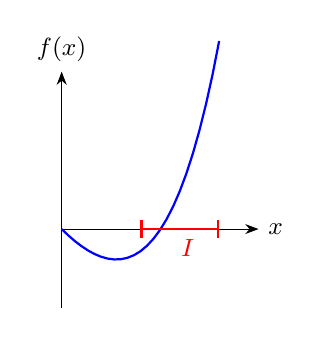
\begin{tikzpicture}
          \draw[->] (0,0) -- (5/2,0) node[right]{$x$};
          \draw[->] (0,-1) -- (0,2) node[above]{$f(x)$}; 
          \draw[blue,thick,domain=0:2] plot(\x, {exp(\x) - 2*\x - 1});
          \draw[|-|,red,thick] (1,0) -- node[pos=.6,below]{$I$} (2,0);
        \end{tikzpicture}
      \end{center}
    \end{column}
    \begin{column}{.5\textwidth}
      Consider the figure to the left.
      Clearly, there is a root of $f$ in the interval $I = [1,2]$.
      \vskip 0.5\baselineskip
      We verify this by calculating
      \[
        f(1) \approx -0.2817 < 0, \quad
        f(2) \approx 2.3891 > 0
      \]
      and noting $f(1)f(2) < 0$.
      \vskip\baselineskip
      Let $\varepsilon = 10^{-1} = 0.1$.
    \end{column}
  \end{columns}
\end{frame}

\begin{frame}{Bisection Method}{Example (continued)}
  Let $I_0 = [a_0,b_0] = [1,2]$.
  Note that
  \[
    \abs{I_0} = \abs{b_0 - a_0} = 1 > 0.1.
  \]
  Midpoint:
  \[
    c_0 = \frac{a_0 + b_0}{2} = \frac{1 + 2}{2} = \frac{3}{2} = 1.5
    \quad\text{with}\quad
    f\!\left(\frac{3}{2}\right) \approx 0.4817.
  \]
  Compare:
  \[
    f(1)f\!\left(\frac{3}{2}\right) < 0, \quad
    f\!\left(\frac{3}{2}\right)f(2) > 0
  \]
  Therefore, $x^* \in [a_0, c_0]$.
\end{frame}

\begin{frame}{Bisection Method}{Example (continued)}
  Set $I_1 = [a_1, b_1] = \left[1,\frac{3}{2}\right] = [a_0, c_0]$.

  Error:
  \[
    \abs{I_1} = \abs{b_1 - a_1}
    = \abs*{\frac{3}{2} - 1}
    = \frac{1}{2}
    = 0.5 
    > 0.1,
  \]
  Midpoint:
  \[
    c_1 = \frac{a_1 + b_1}{2}
    = \frac{1 + \frac{3}{2}}{2}
    = \frac{5}{4}
    = 1.25,
    \quad
    f(c_1) = f\!\left(\frac{5}{4}\right) \approx -9.6570\times 10^{-3}
  \]
  Compare:
  \[
    f(1)f\!\left(\frac{5}{4}\right) > 0, \quad
    f\!\left(\frac{5}{4}\right)f\!\left(\frac{3}{2}\right) < 0
  \]
  Therefore, $x^* \in [c_1, b_1]$.
\end{frame}

\begin{frame}{Bisection Method}{Example (continued)}
  Set $I_2 = [a_2, b_2] = \left[\frac{5}{4}, \frac{3}{2}\right] = [c_1, b_1]$

  Error:
  \[
    \abs{I_2} = \abs{b_2 - a_2}
    = \abs*{\frac{3}{2} - \frac{5}{4}}
    = \frac{1}{4}
    = 0.25 
    > 0.1.
  \]
  Midpoint:
  \[
    c_2 = \frac{a_2 + b_2}{2}
    = \frac{\frac{5}{4} + \frac{3}{2}}{2}
    = \frac{11}{8}
    = 1.375
    \quad
    f(c_2) = f\!\left(\frac{11}{8}\right) \approx 0.2051
  \]
  Compare:
  \[
    f\!\left(\frac{5}{4}\right)f\!\left(\frac{11}{8}\right) < 0, \quad
    f\!\left(\frac{11}{8}\right)f\!\left(\frac{3}{2}\right) > 0
  \]
  Therefore, $x^* \in [a_2, c_2]$.
\end{frame}

\begin{frame}{Bisection Method}{Example (continued)}
  Set $I_3 = [a_3, b_3] = \left[\frac{5}{4}, \frac{11}{8}\right] = [a_2, c_2]$

  Error:
  \[
    \abs{I_3} = \abs{b_3 - a_3}
    = \abs*{\frac{11}{8} - \frac{5}{4}}
    = \frac{1}{8}
    = 0.125 
    > 0.1.
  \]
  Midpoint:
  \[
    c_3 = \frac{a_3 + b_3}{2}
    = \frac{\frac{5}{4} + \frac{11}{8}}{2}
    = \frac{21}{16}
    = 1.3125
    \quad
    f(c_3) = f\!\left(\frac{21}{16}\right) \approx 0.0905
  \]
  Compare:
  \[
    f\!\left(\frac{5}{4}\right)f\!\left(\frac{21}{16}\right) < 0, \quad
    f\!\left(\frac{21}{16}\right)f\!\left(\frac{11}{8}\right) > 0
  \]
  Therefore, $x^* \in [a_3, c_3]$.
\end{frame}

\begin{frame}{Bisection Method}{Example (continued)}
  Set $I_4 = [a_4, b_4] = \left[\frac{5}{4}, \frac{21}{16}\right] = [a_3, c_3]$.

  Error:
  \[
    \abs{I_4} = \abs{b_4 - a_4}
    = \abs*{\frac{21}{16} - \frac{5}{4}}
    = \frac{1}{16}
    = 0.0625
    < 0.1.
  \]
  Midpoint:
  \[
    c_4 = \frac{a_4 + b_4}{2}
    = \frac{\frac{5}{4} + \frac{21}{16}}{2}
    = \frac{41}{32}
    \approx 1.28125, \quad
    f(c_4) = f\!\left(\frac{41}{32}\right) \approx 0.0386
  \]
\end{frame}

\begin{frame}{Bisection Method}{Example (continued)}
  Since $\abs{I_4} = \abs{b_4 - a_4} < \varepsilon$ (the interval length is
  within the specified tolerance), we stop the bisection method.

  The root $x^*$ is approximately $c_4 = 1.28125$, which we also indicate as
  \[
    x^* \approx 1.28125.
  \]
\end{frame}

\begin{frame}{Bisection Method}{Example (continued)}
  Our calculations in this example are quite verbose, we can abbreviate it into
  a table:
  \[
    \begin{array}{|c|c|c|c||c|c|c|}
      \hline
      k & a_k & c_k & b_k & \abs{c_k - c_{k-1}} & \abs{f(c_k)} & \abs{b_k - a_k} \\
      \hline
      0 & 1 & 1.5 & 2 & & 0.4817 & 1 \\
      1 & 1 & 1.25 & 1.5 & 0.25 & 0.0097 & 0.5 \\
      2 & 1.25 & 1.375 & 1.5 & 0.125 & 0.2051 & 0.25 \\
      3 & 1.25 & 1.3125 & 1.375 & 0.0625 & 0.0905 & 0.125 \\
      4 & 1.25 & 1.28125 & 1.3125 & 0.03125 & 0.0386 & 0.0625 \\
      \hline
    \end{array}
  \]
  The last three column indicate the possible error measures for the bisection
  method.

  \textcolor{red}{Can you see the difference between the different possible
  stopping criteria for the bisection method for this example using this table?}
\end{frame}

\section{Analysis}

\begin{frame}{Bisection Method}{Convergence analysis}
  The question arises whether the sequence $(c_k)_{k=0}^\infty$ of
  approximations generated by the bisection method will actually converge to a
  root $x^*$ of $f$.

  That is, will
  \[
    c_k \to x^*
    \quad \text{as} \quad
    k \to \infty?
  \]
  Equivalently, we may ask if
  \[
    \abs{c_k - x^*} \to 0
    \quad \text{as} \quad
    k \to \infty
  \]
  or
  \[
    \abs*{\frac{c_k - x^*}{x^*}} \to 0
    \quad \text{as} \quad
    k \to \infty?
  \]
\end{frame}

\begin{frame}{Bisection Method}{Convergence analysis}
  \begin{columns}[t,onlytextwidth]
    \begin{column}{.4\textwidth}
      \begin{center}
        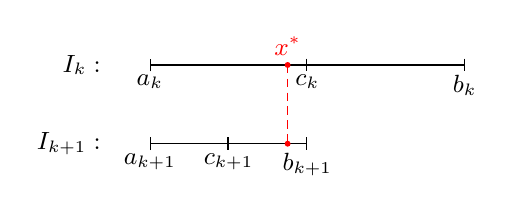
\begin{tikzpicture}
          \draw[|-|] (0,0) -- (2,0) node[below]{$c_k$};
          \draw[-|] (2,0) -- (4,0);
          \node at (0,0)[below]{$a_k$};
          \node at (4,0)[below]{$b_k$};

          \draw[|-|] (0,-1) node[below]{$a_{k+1}$} -- (1,-1) node[below]{$c_{k+1}$};
          \draw[-|] (1,-1) -- (2,-1) node[below]{$b_{k+1}$};

          \node at(7/4,0)[above,red]{$x^*$};
          \filldraw[red] (7/4,0) circle[radius=.3mm];
          \filldraw[red] (7/4,-1) circle[radius=.3mm];
          \draw[densely dashed,red] (7/4,0) -- (7/4,-1);

          \node at(0,0)[left=5mm]{$I_k:$};
          \node at(0,-1)[left=5mm]{$I_{k+1}:$};
        \end{tikzpicture}
      \end{center}
    \end{column}
    \begin{column}{.5\textwidth}
      Consider the figure on the left.
      \vskip\baselineskip
      Note that
      \[
        c_k - a_k = \frac{b_k - a_k}{2} = b_k - c_k
      \]
      and $\abs{c_k - a_k} = \abs{b_k - c_k}$.
      \vskip\baselineskip
      Therefore, we may speak of either subinterval $I_k = [a_k, c_k]$ or $I_k =
      [c_k, b_k]$ in the following analysis without loss of generality.
    \end{column}
  \end{columns}
\end{frame}

\begin{frame}{Bisection Method}{Convergence analysis}
  Note that we may write
  \[
    c_k = \frac{a_k + b_k}{2}
    = a_k + \frac{b_k - a_k}{2}.
    %= b_k - \frac{b_k - a_k}{2}.
  \]
  Consider
  \[
    c_k = \frac{a_k + b_k}{2}
    = a_k + \frac{b_k - a_k}{2}.
  \]
  %and rewrite it as
  %\begin{align*}
  %  c_k - a_k &= \frac{b_k - a_k}{2} \\
  %  c_k - x^* + x^* - a_k &= \frac{b_k - a_k}{2} \\
  %  c_k - x^* &= a_k + \frac{b_k - a_k}{2} - x^* \\
  %  &= \frac{a_k + b_k}{2} - x^*
  %\end{align*}
%\end{frame}
%
%\begin{frame}{Bisection Method}{Convergence analysis}
  Subtract $x^*$ on both sides and take the absolute value
  \[
    \abs{c_k - x^*} %= \abs*{\frac{a_k + b_k}{2} - x^*}
    = \abs*{a_k + \frac{b_k - a_k}{2} - x^*} 
    \leq \abs*{a_k - x^*} + \abs*{\frac{b_k - a_k}{2}}
    \leq \frac{\abs{b_k - a_k}}{2} + \frac{\abs{b_k - a_k}}{2}.
  \]
  Hence,
  \[
    \abs{c_k - x^*} \leq \abs{b_k - a_k}.
  \]
\end{frame}

\begin{frame}{Bisection Method}{Convergence analysis}
  Next, we show that
  \[
    \abs{b_k - a_k} \leq \frac{\abs{b - a}}{2^k}.
  \]
  \vskip\baselineskip
  \begin{columns}[t,onlytextwidth]
    \begin{column}{.4\textwidth}
      \begin{center}
        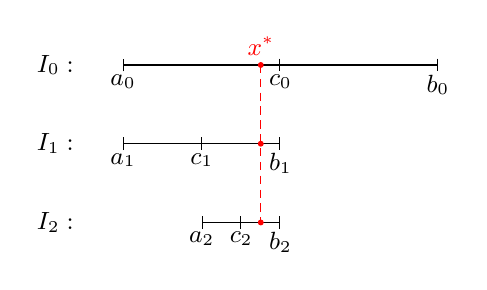
\begin{tikzpicture}
          \draw[|-|] (0,0) -- (2,0) node[below]{$c_0$};
          \draw[-|] (2,0) -- (4,0);
          \node at (0,0)[below]{$a_0$};
          \node at (4,0)[below]{$b_0$};

          \draw[|-|] (0,-1) node[below]{$a_1$} -- (1,-1) node[below]{$c_1$};
          \draw[-|] (1,-1) -- (2,-1) node[below]{$b_1$};

          \draw[|-|] (1,-2) node[below]{$a_2$} -- (3/2,-2) node[below]{$c_2$};
          \draw[-|] (3/2,-2) -- (2,-2) node[below]{$b_2$};

          \node at(7/4,0)[above,red]{$x^*$};
          \filldraw[red] (7/4,0) circle[radius=.3mm];
          \filldraw[red] (7/4,-1) circle[radius=.3mm];
          \filldraw[red] (7/4,-2) circle[radius=.3mm];
          \draw[densely dashed,red] (7/4,0) -- (7/4,-1) -- (7/4,-2);

          \node at(0,0)[left=5mm]{$I_0:$};
          \node at(0,-1)[left=5mm]{$I_1:$};
          \node at(0,-2)[left=5mm]{$I_2:$};
        \end{tikzpicture}
      \end{center}
    \end{column}
    \begin{column}{.5\textwidth}
      Note, with the help of the figure to the left, that
      \[
        \abs{I_1} = \frac{\abs{I_0}}{2}
        \quad \text{and} \quad
        \abs{I_2} = \frac{\abs{I_1}}{2},
      \]
      where $\abs{I_k}$ represents the length of the $k$th subinterval.
      It follows that
      \[
        \abs{I_2} = \frac{\abs{I_1}}{2} 
        = \frac{1}{2}\left(\frac{\abs{I_0}}{2}\right)
        = \frac{\abs{I_0}}{2^2}.
      \]
    \end{column}
  \end{columns}
\end{frame}

\begin{frame}{Bisection Method}{Convergence analysis}
  More generally, after $k$ iterations of the bisection method, we have
  \begin{align*}
    \abs{I_k} &= \frac{\abs{I_{k-1}}}{2} \\
    &= \frac{1}{2}\left(\frac{\abs{I_{k-2}}}{2}\right)
    = \frac{\abs{I_{k-2}}}{2^2} \\
    &= \frac{1}{2^2}\left(\frac{\abs{I_{k-3}}}{2}\right)
    = \frac{\abs{I_{k-3}}}{2^3} \\
    &\;\;\vdots \\
    &= \frac{1}{2^{k-1}}\left(\frac{\abs{I_{0}}}{2}\right)
    = \frac{\abs{I_0}}{2^k}.
  \end{align*}
  %where $\abs{I_0} = \abs{b - a}$ (the length of the original interval).
\end{frame}

\begin{frame}{Bisection Method}{Convergence analysis}
  Hence,
  \[
    \abs{b_k - a_k} = \frac{\abs{b - a}}{2^k}
  \]
  and
  \[
    \abs{c_k - x^*} \leq \frac{\abs{b - a}}{2^k}.
  \]
  We have proved the following
  %\begin{theorem}
  %  Let $[a,b] \subset \mathbb{R}$, where $a < b$, and let $f : [a,b] \to
  %  \mathbb{R}$ be a function.
  %  If $f$ is continuous on $[a,b]$ and $f(a)f(b) < 0$, then there exists $x^*
  %  \in (a,b)$ such that $f(x^*) = 0$ and $\lim_{k \to 0} c_k = x^*$, where
  %  sequence $\left(c_k\right)_{k=0}^\infty$ is generated by the bisection
  %  method.
  %\end{theorem}
  \begin{theorem}
    Let $[a,b] \subset \mathbb{R}$, where $a < b$, and let $f : [a,b] \to
    \mathbb{R}$ be a function such that $f$ is continuous on $[a,b]$ and
    $f(a)f(b) < 0$.
    The bisection method generates a sequence $\left(c_k\right)_{k=0}^\infty$
    that approximates a root $x^*$ of $f$ in $[a,b]$ with the property that
    \vskip -.5em
    \[
      \abs{c_k - x^*} \leq \frac{\abs{b - a}}{2^k}, \quad
      k \in \mathbb{N}.
    \]
    \vskip -.5em
  \end{theorem}
\end{frame}

%\begin{frame}{Bisection Method}{Convergence analysis}
%  The bisection method generates a sequences of \emph{nested intervals}:
%  \[
%    I_{k+1} \subset I_k, \quad
%    k\in\{0,1,2,\dotsc\}
%  \]
%  Under certain assumptions and with a bit of work\footnote{This can be proved
%  using knowledge of Real Analysis (MAT01A3).}, one can prove that if
%  $(I_k)_{k=0}^\infty$ is a sequence of nested intervals, then there exists an
%  $x^* \in \mathbb{R}$ such that 
%  \[
%    x^* \in \displaystyle\bigcap_{k=0}^\infty I_k,
%  \]
%  where $\bigcap_{k=0}^\infty I_k$ indicates the intersection of all the
%  intervals $I_k$.
%  Hence, the bisection method will converge to a root $x^*$ of $f$,
%  provided that the $x^* \in I_0$.
%\end{frame}

\begin{frame}{Bisection Method}{Convergence analysis}
  This theorem allows us to calculate the number of iterations to achieve a
  specified tolerance $\varepsilon$.

  Suppose
  $
  %\[
    \dfrac{\abs{b - a}}{2^k} \leq \varepsilon.
  %\]
  $
  Taking the natural logarithm\footnote{We could also take the logarithm
  (base 10).} on both sides yields
  \begin{alignat*}{4}
    \ln\left(\frac{\abs{b - a}}{2^k}\right) &\leq \ln(\varepsilon) 
    \quad &
    &\implies \quad&
    \ln(\abs{b - a}) - \ln(2^k) &\leq \ln(\varepsilon) \\
    &&&\implies & -k\ln(2) &\leq \ln(\varepsilon) - \ln(\abs{b - a}) \\
    &&&\implies & -k &\leq \frac{\ln(\varepsilon) - \ln(\abs{b - a})}{\ln(2)}
    \\
    &&&\implies & k &\geq \frac{\ln(\abs{b - a}) - \ln(\varepsilon)}{\ln(2)}
  \end{alignat*}
\end{frame}

\begin{frame}{Bisection Method}{Convergence analysis}
  The expression
  \begin{equation} \label{eq:iter-calc-formula}
    k \geq \frac{\ln(\abs{b - a}) - \ln(\varepsilon)}{\ln(2)}
    = \frac{\ln\left(\abs{b - a}/\varepsilon\right)}{\ln(2)}
  \end{equation}
  informs us the \emph{minimum required number of iterations} that should be
  performed to achieve the specified tolerance $\varepsilon$.

  However, the expression $\ln(\abs{b - a}/\varepsilon)/\ln(2)$ in
  \eqref{eq:iter-calc-formula}
  %\[
  %  \frac{\ln(\abs{b - a}/\varepsilon)}{\ln(2)}
  %\]
  will usually evaluate to a real number,
  so we have to choose the next largest natural number.

  \begin{block}{Note}
    The inequality \eqref{eq:iter-calc-formula} requires no information about $f$
    itself.
  \end{block}
\end{frame}

\begin{frame}{Bisection Method}{Convergence analysis}
  \begin{example}
    Consider the function and interval given in Example
    \ref{ex:bisection-method-1}.
    Determine the number of iterations required by the bisection method if the
    given tolerance is $\varepsilon = 10^{-1}$.
  \end{example}
  We have
  \[
    a_0 = 0, \quad
    b_0 = 2, \quad
    \varepsilon = 10^{-1}.
  \]
  Substituting these values into \eqref{eq:iter-calc-formula}, we obtain
  \[
    k \geq \frac{\ln(\abs{1 - 0}) - \ln(10^{-1})}{\ln(2)} \approx 3.3219.
  \]
  We therefore choose $k = 4$.
\end{frame}

\begin{frame}{Bisection Method}{Convergence analysis}
  \begin{example}
    Suppose $f$ is a function with a root in $[0,2]$ and that $f(0)f(2) < 0$.
    Determine the number of iterations required by the bisection method if the
    given tolerance is $\varepsilon = 10^{-5}$.
  \end{example}
  We have
  \[
    a_0 = 0, \quad
    b_0 = 2, \quad
    \varepsilon = 10^{-5}
  \]
  and
  \[
    k \geq \frac{\ln(\abs{2 - 0}) - \ln(10^{-5})}{\ln(2)} \approx 17.60964
    \quad \implies \quad
    k = 18.
  \]
\end{frame}

\begin{frame}{Bisection Method}{Order and rate of convergence}
  In numerical analysis we are often concerned with \emph{how quickly a
  numerical method approximates a solution} (or \emph{how quickly a numerical
  method theoretically converges to a solution if $k \to \infty$}).

  A quantitative measure of convergence is the order and rate of convergence.
  \begin{definition}
    The \emph{order of convergence} of an iterative method is the quantity
    $\alpha$ such that
    \begin{equation} \label{eq:convergence-order-rate-def}
      \lim_{k\to\infty} \frac{\abs{x_{k+1} - x^*}}{\abs{x_k - x^*}^\alpha} =
      \mu,
    \end{equation}
    where $\mu$ is called the \emph{rate of convergence} (or \emph{asymptotic
    rate of convergence}).
  \end{definition}
\end{frame}

\begin{frame}{Bisection Method}{Order and rate of convergence}
  Order and rate of convergence is usually determined by \emph{error
  analysis}\footnote{See slides \ref{fr:abs-rel-error}--\ref{fr:comp-error} for
  definitions of the various errors we encounter in numerical analysis.}
  we investigate how errors between subsequent steps of a numerical are related
  to each other, or how the errors are related to the initial error.

  For the bisection method, we have
  \[
    \frac{e_{k+1}}{e_k}
    =\frac{\abs{c_{k+1} - x^*}}{\abs{c_k - x^*}} = \frac{1}{2}.
  \]
  Therefore, $\alpha = 1$ and $\mu = \frac{1}{2}$.
  We say that the bisection method converges \emph{linearly}\footnote{Because $\alpha =
  1$.}.
\end{frame}

%\begin{frame}{Bisection Method}{Order and rate of convergence}
%  To wit,
%  \[
%    \abs{c_{k+1} - x^*} = \abs*{\frac{b_0 - a_0}{2^{k+1}} - x^*}, \quad
%    \abs{c_k - x^*} = \abs*{\frac{b_0 - a_0}{2^k} - x^*}
%  \]
%  and therefore
%  \begin{align*}
%    \frac{\abs{c_{k+1} - x^*}}{\abs{c_k - x^*}}
%    = \frac{\abs*{\frac{b_0 - a_0}{2^{k+1}} - x^*}}{\abs*{\frac{b_0 - a_0}{2^k}
%    - x^*}}
%    = \abs*{\frac{\frac{b_0 - a_0}{2^{k+1}} - x^*}{\frac{b_0 - a_0}{2^k}
%    - x^*}}
%    &= \abs*{\frac{b_0 - a_0 - 2^{k+1}x^*}{2^{k+1}}\,\frac{2^k}{b_0 -
%    a_0 - 2^kx^*}} \\
%    &= \frac{1}{2}\abs*{\frac{b_0 - a_0 - 2^{k+1}x^*}{b_0 - a_0 - 2^kx^*}}
%  \end{align*}
%\end{frame}

\begin{frame}{Exercises}
\end{frame}

\begin{frame}{Exercises}
\end{frame}

\begin{frame}{Questions To Ponder}
  \begin{itemize}
    \item What happens with the bisection method when we remove assumptions
      (e.g., continuity of $f$, root in $[a,b]$, etc.)?
    \item What if there are multiple roots of $f$ in the interval $[a,b]$?
    \item Are there root-finding methods which converge to a root quicker than
      the bisection method?
    \item What is the difference between accuracy, precision and tolerance in
      the context of numerical methods?
  \end{itemize}
\end{frame}

\begin{frame}{Further Reading}
  \nocite{burden2015numerical}
  \printbibliography
\end{frame}

\appendix
\section{Errors and Stopping Criteria}
\begin{frame}{Stopping Criteria} \label{fr:stopping-criteria}
  A \emph{stopping criterion} (plural: \emph{stopping criteria}) is a logical
  and mathematical test performed to see whether a numerical method is
  terminated or not.

  To facilitate a discussion around this, we introduce the error concepts
  encountered in the study of applied mathematics and numerical analysis.

  First, we introduce two ways in which we can measure error: \emph{absolute
  error} and \emph{relative error}.

  Then we look at the three types of error encountered in computation:
  \emph{numerical error}, \emph{truncation error}, and \emph{computational
  error}.
\end{frame}

\begin{frame}{Absolute and Relative Error} \label{fr:abs-rel-error}
  \begin{definition}[Absolute Error]
    The \emph{absolute error} between an actual/solution value $x$ and its
    approxmation $\hat{x}$ is given by
    \begin{equation} \label{eq:abs-error}
      e_\text{abs} = \abs{x - \hat{x}}.
    \end{equation}
  \end{definition}
  \begin{definition}[Relative Error]
    The \emph{relative error} between an actual/solution value $x$ and its
    approximation $\hat{x}$ is given by
    \begin{equation} \label{eq:rel-error}
      e_\text{rel} = \abs*{\frac{x - \hat{x}}{x}}.
    \end{equation}
  \end{definition}
\end{frame}

\begin{frame}{Bisection Method}{Absolute and Relative Error}
  Relative error is invariant to scaling (of the values):
  \[
    \abs*{\frac{(\lambda x) - (\lambda \hat{x})}{\lambda x}}
    = \abs*{\frac{\lambda (x - \hat{x})}{\lambda x}}
    = \abs*{\frac{x - \hat{x}}{x}}.
  \]
  Relative error expresses the absolute error as a fraction of actual/solution
  value, and represents absolute error's significance compared to the magnitude
  of the actual/solution value.

  Relative error is closely related to \emph{percentage error}:
  \[
    e_{\text{percentage}} = e_{\text{rel}} \times 100\%.
  \]
  Relative and percentage error are useful when the solution magnitudes vary a
  lot.
\end{frame}

\begin{frame}{Numerical, Truncation and Computational Error}{Numerical error}
  Let $x$ be our actual/solution value and $\hat{x}$ be our approximation of
  this value.

  Numerical error is the difference between the solutions of our mathematical
  model (what we have been calling the solution previously) and the solution of
  the numerical model (what we have been calling the approximations generated by
  the numerical method previously).

  It is quantitatively measured by either the absolute error
  \eqref{eq:abs-error} or relative error \eqref{eq:rel-error}.
\end{frame}

\begin{frame}{Numerical, Truncation and Computational Error}{Truncation error}
  \label{fr:trunc-error}
  Most real numbers may be represented as a decimal number with an infinite
  number of digits after the decimal point.
  For example,
  \[
    \pi = 3.141592653589793...
  \]

  However, computing devices (calculators, cellphones, laptops, desktop personal
  computers, etc.) only have finite memory to represent numbers.
  These devices tend to truncate (chop off) or round numbers which are larger
  than the available memory.
  For example,
  \[
    \hat{\pi} = 3.14159.
  \]

  This difference between the actual number representation and
  round-off/truncated number is called the \emph{truncation error} (or
  \emph{round-off error}).
\end{frame}

\begin{frame}{Numerical, Truncation and Computational Error}{Truncation error}
  \label{fr:trunc-error-taylor-series}
  Truncation error will also be encountered in numerical methods derived from
  Taylor series of a function $f$ about a point $x_0$:
  \[
    f(x) = \sum_{k = 0}^\infty \frac{f^{(k)}(x_0)}{k!}(x - x_0)^k.
  \]
  In practice, we use a finite number of terms in the above series to obtain the
  $p$th-degree Taylor polynomial:
  \begin{align*}
    T_f(x) &= \sum_{k = 0}^p \frac{f^{(k)}(x_0)}{k!}(x - x_0)^k \\
    &= f(x_0) + f'(x_0)(x - x_0) + \frac{f''(x_0)}{2!}(x - x_0)^2 + \dotsb +
    \frac{f^{(p)}(x_0)}{p!}(x - x_0)^p.
  \end{align*}
\end{frame}

\begin{frame}{Numerical, Truncation and Computational Error}{Computational error}
  \label{fr:comp-error}
  The \emph{computational error} $e_c$ is the sum of the numerical error $e_n$
  and truncation error $e_r$:
  \[
    e_c = e_n + e_r.
  \]
  This represents the total error between any analytical process and our
  computational and numerical approximation processes.
\end{frame}

\begin{frame}{Stopping Criteria}{Difference-based errors and stopping criteria}
  One of the disadvantages of the absolute error \eqref{eq:abs-error} and
  relative error \eqref{eq:rel-error} is that the definitions require the actual
  solution of the problem---which, in practice, is not known ahead of time or at
  all.

  Most numerical methods use \emph{difference-based errors} as stopping
  criteria:
  \begin{align}
    \abs{x_k - x_{k-1}} &< \varepsilon, \label{eq:diff-error-abs}\\
    \frac{\abs{x_k - x_{k-1}}}{\abs{x_k}} &< \varepsilon. 
    \label{eq:diff-error-rel}
  \end{align}
  Examples were already encountered in \eqref{eq:stop-crit-abs-error} and
  \eqref{eq:stop-crit-rel-error}.
\end{frame}

\begin{frame}{Stopping Criteria}{Difference-based errors and stopping criteria}
  \textcolor{red}{What is the difference between $\abs{x_k - x^*}$ and $\abs{x_k
  - x_{k-1}}$? Is any accuracy lost?}

  Suppose we have a linearly convergent numerical method (for example, such as
  the bisection method): $\abs{e_k} \leq q\abs{e_{k-1}}$ (with $0 < q < 1$).
  %\[
  %  \abs{e_k} \leq q\abs{e_{k-1}}, \quad 0 < q < 1
  %\]
  %Let $x_k = x^* - e_k$, where $e_k$ represents the error
  
  Then
  \begin{align*}
    \abs{x_k - x_{k-1}} = \abs{x_k - x^* + x^* - x_{k-1}}
    = \abs{e_k - e_{k-1}} 
    &\geq \bigl\lvert{\abs{e_k} - \abs{e_{k-1}}}\bigr\rvert \\
    &\geq \abs{e_k} - \abs{e_{k-1}} \\
    &\geq \abs{e_k} - \frac{1}{q}\,\abs{e_k} \\
    &= \frac{q - 1}{q}\,\abs{e_k}
    %\leq \abs{e_k} + \abs{e_{k-1}}
    %\leq \abs{e_k} + q\abs{e_k}
    %= (1 + q)\abs{e_k}
  \end{align*}
\end{frame}

\begin{frame}{Stopping Criteria}{Difference-based errors and stopping criteria}
  Hence, we have shown that
  \[
    \abs{e_k} \leq \frac{q}{q - 1}\,\abs{x_k - x_{k-1}}.
  \]
  The absolute error $\abs{e_k} = \abs{x_k - x^*}$ is bounded above by the
  difference-based error $\abs{x_k - x_{k-1}}$.
  If $\abs{x_k - x_{k-1}} < \varepsilon$, then we shall have $\abs{e_k} =
  \abs{x_k - x^*} < \varepsilon$.

  \begin{block}{Note}
    This analysis is only applicable to this specific case (linear convergence
    and $0 < q < 1$) and not in general.
    It serves to illustrate why we may use difference-based error rather than an
    error involving the actual solution $x^*$.
  \end{block}
\end{frame}

\end{document}
